% !TEX root = ../MemPod.tex
\section{Architecture}
\label{sec:Architecture}

Our clustered migration mechanism is designed to address key challenges associated with the migration problem. In this section, we present a complete description of our micro-architectural design, followed by a breakdown of the important design decisions, along with the corresponding challenge addressed by each one.

%\begin{table*}[t]
%\begin{tabularx}{\textwidth}{ |X|X|X|X|X| }
%  \hline
%    \textbf{Challenge} & \textbf{Tradeoff} & \textbf{THM} & \textbf{HMA} & \textbf{MemPod} \\ \hline       
%    Page Relocation & Flexibility / Time & Only 1 candidate \newline (Minimum / Very low)& No restrictions \newline (Max / High) & Intra-Pod migration \newline (High / Medium) \\ \hline
%    Remap Table Size & Flexibility / Area & 1 entry per fast page \newline \textasciitilde2.4MB \newline (Minimum / Medium) & No remap table \newline 0 Bytes \newline (Max / Min) & 1 entry per fast page \newline 4.5MB (1.125MB/Pod) \newline (High / Medium) \\ \hline
%    Activity Tracking & Accuracy / Area & 8 bits per fast page \newline 64kB \newline (Medium / Low) & 16 bits per page \newline 1.125MB \newline (Max / Max) & 48 bits per fast page \newline 384kB \newline (High / Medium)\\ \hline
%    Migration Trigger & N/A & Threshold based & Interval based & Interval based\\ \hline
%    Tracking Organization & Simplicity / Parallelization & Fully Centralized \newline Serialized requests \newline (High / Min) & Fully distributed \newline (High / Max) & Semi-distributed \newline Pods operate independently \newline (High / High)\\ \hline
%    Migration Driver & Communication cost & CPU \newline High latency \newline (Max) & CPU (OS) \newline High latency \newline (Max) & Pod \newline Very low latency \newline (Low)\\ \hline
%    Migration Cost & Time & HW cost + communication \newline (Medium) & HW + SW + cold TLBs \newline (Max) & HW cost \newline (Min)\\ \hline
%\end{tabularx}
%  \caption{Breakdown of state-of-the-art designs}
%  \label{tab:comparison}
%\end{table*}

\begin{table}
  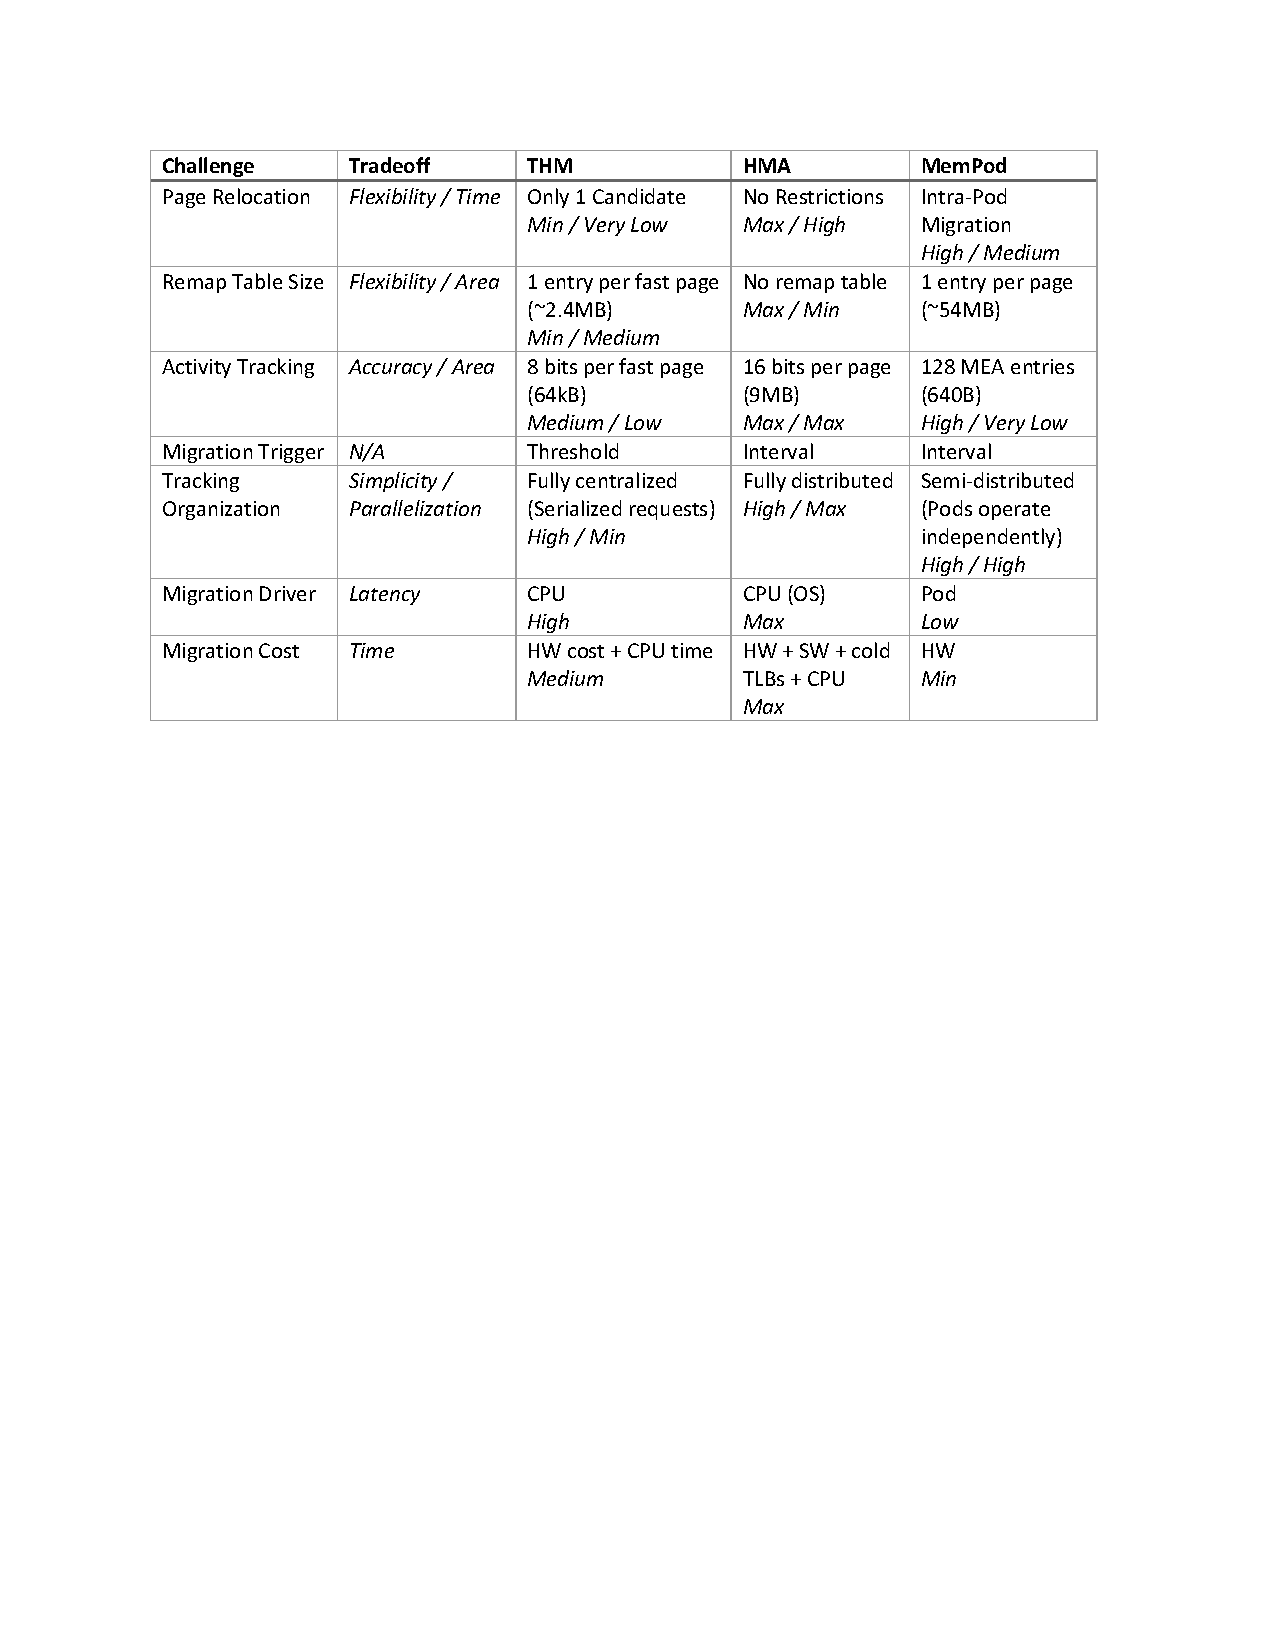
\includegraphics[width=\linewidth]{figures/comparison_table.pdf}
  \caption{Breakdown of state-of-the-art designs}
  \label{tbl:breakdown}
\end{table}

\subsection{Clustered Migration Architecture}

 Figure \ref{fig:architecture_complete} presents an overview of MemPod. MemPod's design was kept modular to facilitate system integration and scalability. A number of memory ``Pods'' are injected between the LLC and the system's memory controllers (MCs). Each Pod clusters a number of MCs and enforces migrations to only occur among its member MCs. Pods do not communicate with each other, preventing inter-Pod migrations. To the rest of the system, Pods are exposed as MCs. With MemPod's transparent design, each Pod will now be receiving all the requests originally addressed to any of the Pod's member MCs. 
 
\begin{figure}
 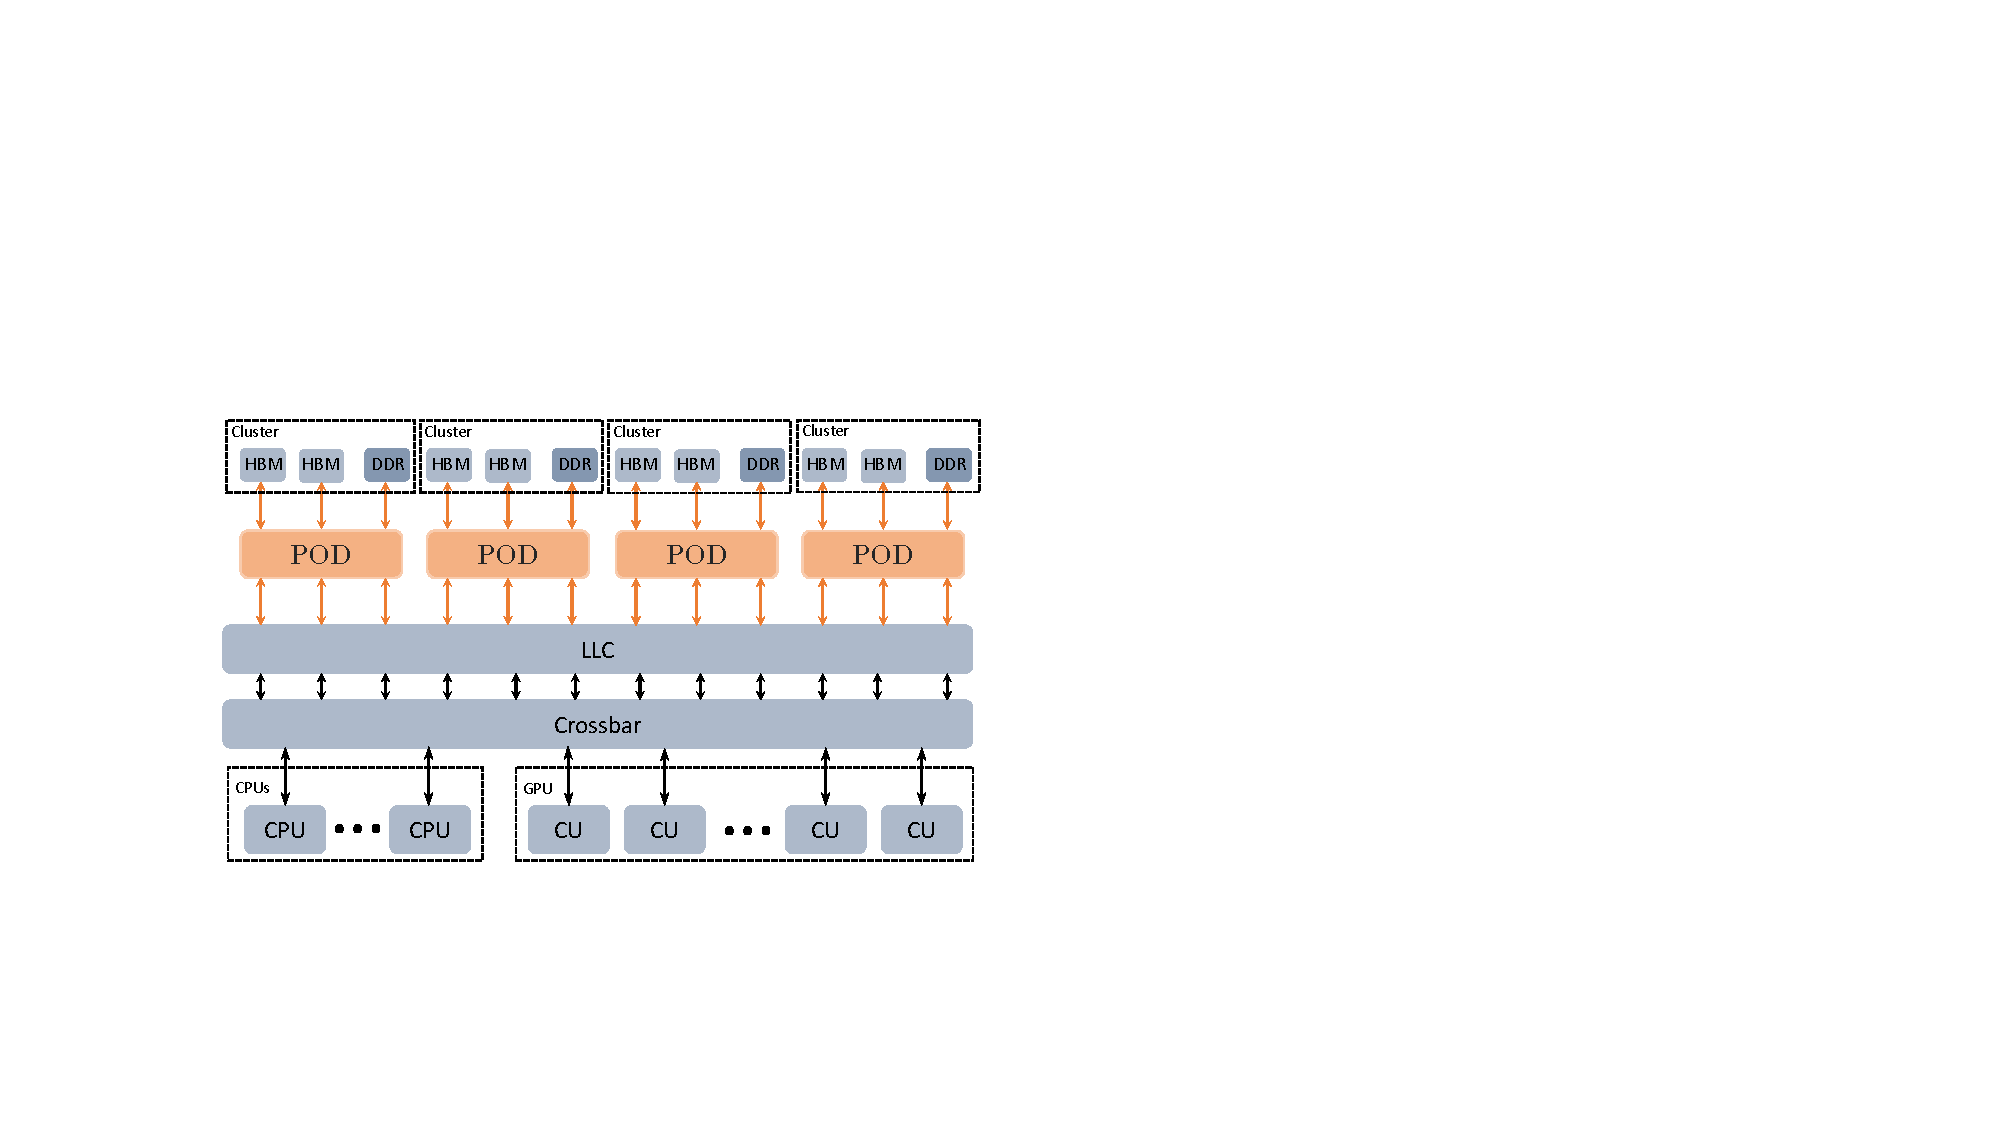
\includegraphics[width=0.47\textwidth]{figures/mempod_org.pdf}
 \caption{MemPod high-level architecture}
 \label{fig:architecture_complete}
\end{figure}

\remark{Very confused by the figure.  Why are there 3 channels from a POD to 
the LLC?  Why are there 12 channels from LLC to the crossbar?  Why are there
no communication paths between memory controllers of the same pod -- I thought
that was the main point?  I can't tell where the migration traffic would 
actually go in this picture, there is no path between them.  Figure 5
also shows no paths between memory channels.\\A.P.: Updated the figures. Figure 5(b) might be too complicated. What do you think?}

\remark{Also still confused why if you're assuming 1 HBM to 8 DDR pages,
why we keep showing 2 HBM MCs and 1 DDR.\\A.P.: The number of MCs is irrelevant to capacity (and number of pages). We simulate a 1:8 memory ratio, but we have 8 HBM MCs for the 1GB of HBM and 4 MCs for the 8GB of DDR4. Based on the JEDEC HBM specs and the high price of adding pins this should be a realistic configuration.}

When a memory request arrives, the pod monitors the request, updates any 
necessary migration-related activity tracking counters, and forwards 
the request to the intended recipient MC. The migration logic within a Pod does not need to be invoked during a response from any MC and can be bypassed to reduce memory access latency. A drawback of clustering MCs into Pods is the serialization of potentially parallel requests to different MCs of a single Pod. As such, activity tracking within a Pod as well as the subsequent forwarding of requests must be as efficient as possible. 

MemPod's clustered architecture also aids in reducing global traffic during migrations compared to non-partitioned mechanisms.  Because migration
traffic happens within a pod, this architecture significantly reduces global
traffic and enables highly parallel migrations.
%  Higher global traffic could require the global switch (or crossbar) to have higher bandwidth resulting in increased energy costs and could also introduce performance penalties. Furthermore, with Pods servicing migrations transparently, the system's CPUs will be able to keep executing non-memory instructions during migrations. 

\subsubsection*{Memory Pod}

The major architectural elements of a Pod are shown in Figure \ref{fig:architecture_pod}. A Pod includes an activity tracking (MEA) unit, a remap table for keeping track of migrated pages and a forwarding unit that can re-encode a request with the relay address and, based on that address, send the request to the appropriate MC.
%
%\begin{figure}[h]
%  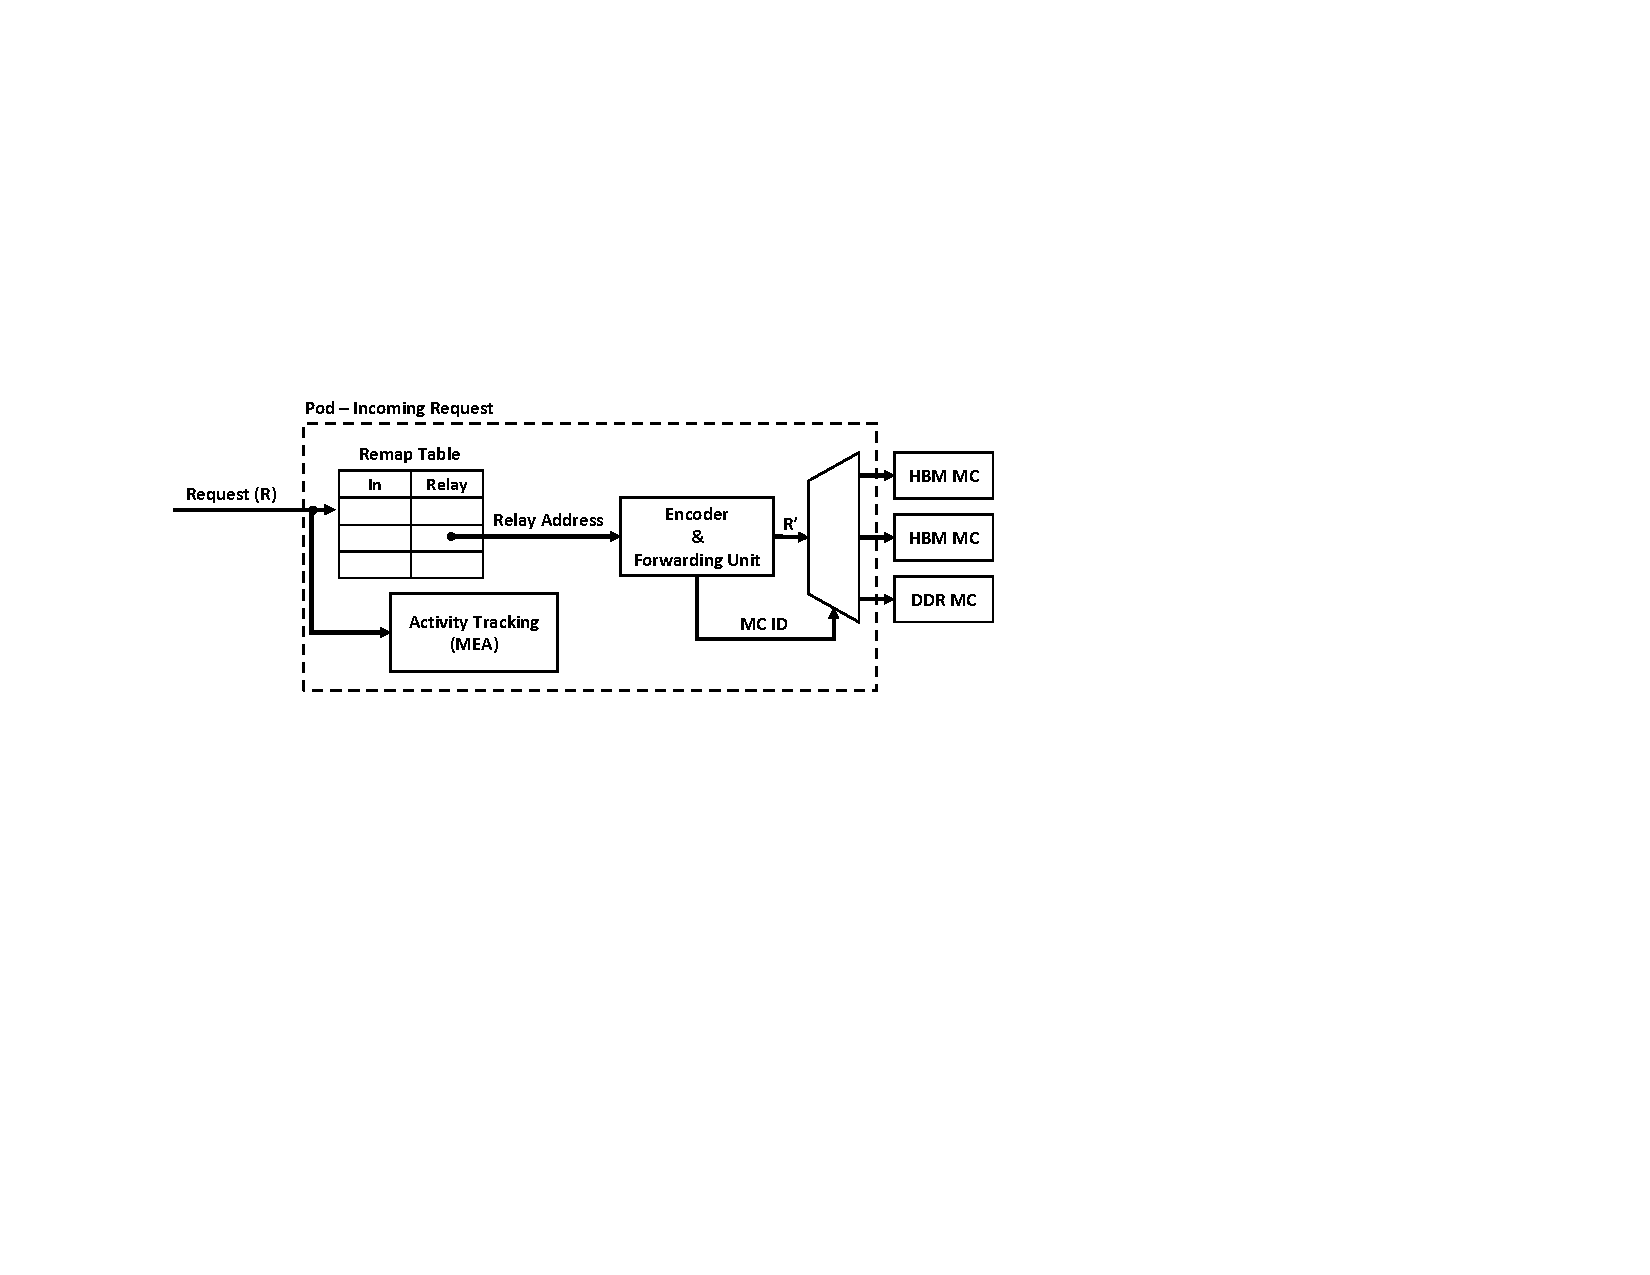
\includegraphics[width=0.46\textwidth]{figures/pod_design_request.pdf}
%  \caption{Major architectural Pod elements}
%  \label{fig:architecture_pod}
%\end{figure}

\begin{figure}
\begin{subfigure}{0.46\textwidth}
  \centering
  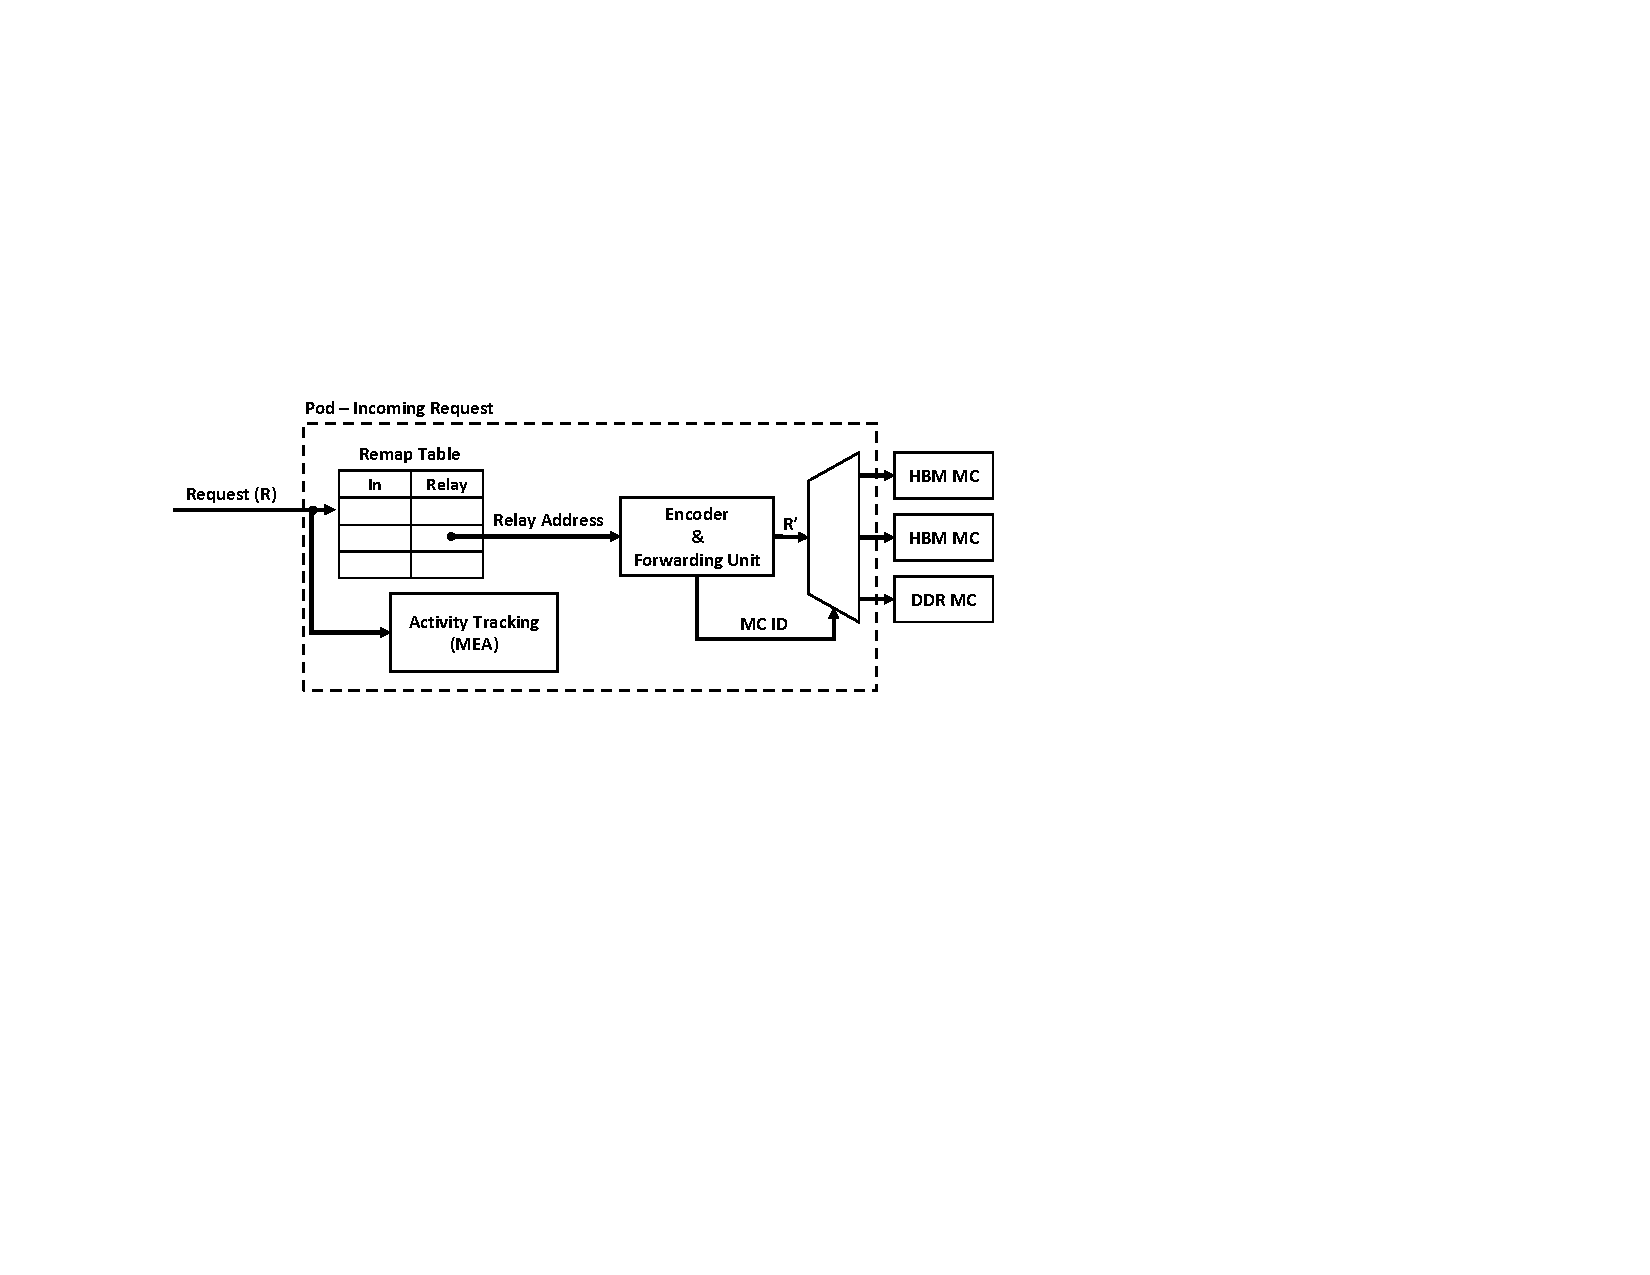
\includegraphics[width=\textwidth]{figures/pod_design_request.pdf}
  \caption{Pod's request forwarding operation}
\end{subfigure}%

\begin{subfigure}{0.46\textwidth}
  \centering
  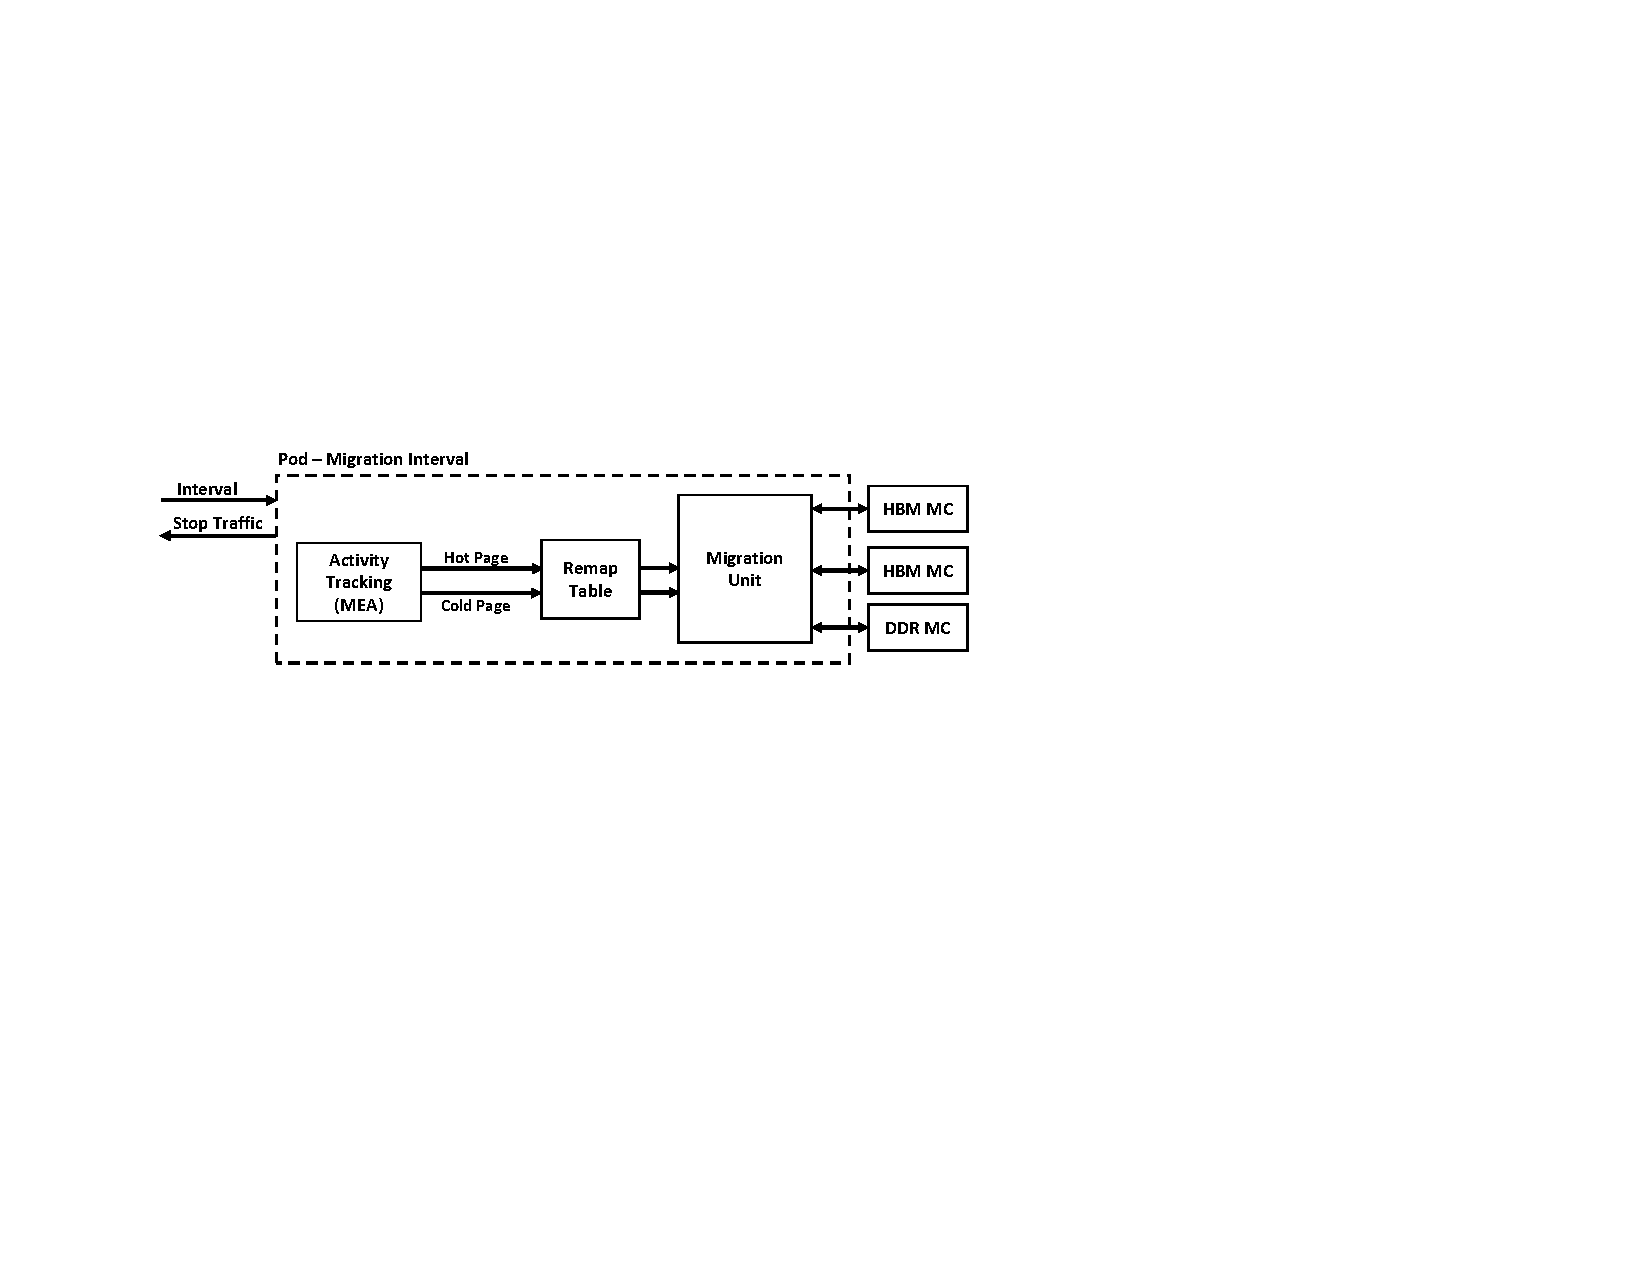
\includegraphics[width=\textwidth]{figures/pod_design_migration.pdf}
  \caption{Pod's migration procedure}
\end{subfigure}
\caption{Major architectural Pod elements}
\label{fig:architecture_pod}
\end{figure}

\remark{Don't like footnotes -- only use if desperate.  If it's important,
put in the text.  If it isn't, don't include it.}
A designer can vary the parallelism and flexibility of MemPod by varying the
number of pods. A design with one pod is equivalent to a centralized 
migration controller allowing any-to-any migration,
%\footnote{Any-to-any migration: page migration without constraints on source and destination. All MCs can migrate a page to any other MC.}, 
while a design with a pod number equal to the number of MCs would imply that migration is disabled. A reasonable design point would be to set the number of Pods equal to the number of slow-memory MCs. Such a configuration inherently restricts migration between slow off-chip channels, while at the same time maintaining full channel-level parallelism on the system's bottleneck: the slow MCs. In a configuration where the number of fast-memory MCs are not a multiple of slow-memory MCs, Pods can be configured asymmetrically or some MCs could be members of multiple Pods, with their capacity partitioned to avoid crosstalk issues. In Figure \ref{fig:architecture_complete} we present a system with eight MCs for the fast, on-die stacked memory and four MCs for the slow off-chip memory. Throughout this paper we use die-stacked HBM as the fast memory \cite{JEDEC-HBM-REVISED} and DDR4-1600 as our off-chip memory. The use of four pods imposes few restrictions on migration possibilities, while forbiding migration between two slow-memory channels without any additional logic. For the remainder of this paper, we set the number of pods to four.

The design of a complete memory manager can be broken down into the following 5 ``building blocks'':
\begin{description}[style=unboxed,leftmargin=0cm]
\setlength\itemsep{0em}
\item [Migration flexibility:] Defines which areas in memory can be used as migration candidates. Higher flexibility offers more potential for performance improvement and increases book-keeping cost.
\item [Remap table:] A structure that keeps track of migrated pages and is able to provide a relay address given a requested address.
\item [Activity tracking:] Logic and structures needed to profile memory requests and predict future ``hot'' pages.
\item [Migration trigger:] Defines when migration occurs. Usually the trigger can be interval-based or threshold-based.
\item [Migration driver/datapath:] Defines the path followed and the hardware modules involved in performing migrations.
\end{description}

\subsection{Building Blocks}

Each of the above building blocks introduces some trade-off. For example, allowing more flexibility in migration locations can lead to higher performance benefits, at the cost of larger book-keeping structures. Table \ref{tbl:breakdown} shows a comparison of each mechanism's elements. The following subsections provide a detailed description of each building block. For each block, we present MemPod's, THM's and HMA's approach, as well as alternative designs found in the literature. The design choices for the various building blocks are largely
orthogonal.  Thus, we describe each separately, with description of the options
and tradeoffs.

\subsubsection{Page Relocation and Remap Table Size}
\label{sec:relocation}

Migrating pages can provide the highest benefit when no restrictions are imposed on the available migration locations.  This amount of flexibility, however,
requires more bookkeeping and can incur a higher cost.

A hardware-driven migration mechanism requires some kind of remap table,
commonly implemented as a hash structure, indexed by a page's address and pointing to the migrated (or relay) page address if one exists. On a page migration, the remap table is updated to reflect the new address of a migrated page. 

The remap table should provide the remap, or relay, address for each original
page address.  Some other structures may also be necessary to avoid expensive
table searches when an inverse lookup is needed (e.g., to identify pages
currently mapped to slow or fast memory).

\ignore{
However, a ``naive'' remap table design can fail when re-migration of pages is allowed. A content-aware remap table is necessary in order to support re-migration. Figure \ref{fig:remap_table_comparison} presents a side-by-side comparison of the operation of these two tables and demonstrates how a naive table can fail.

\begin{figure}[h]
  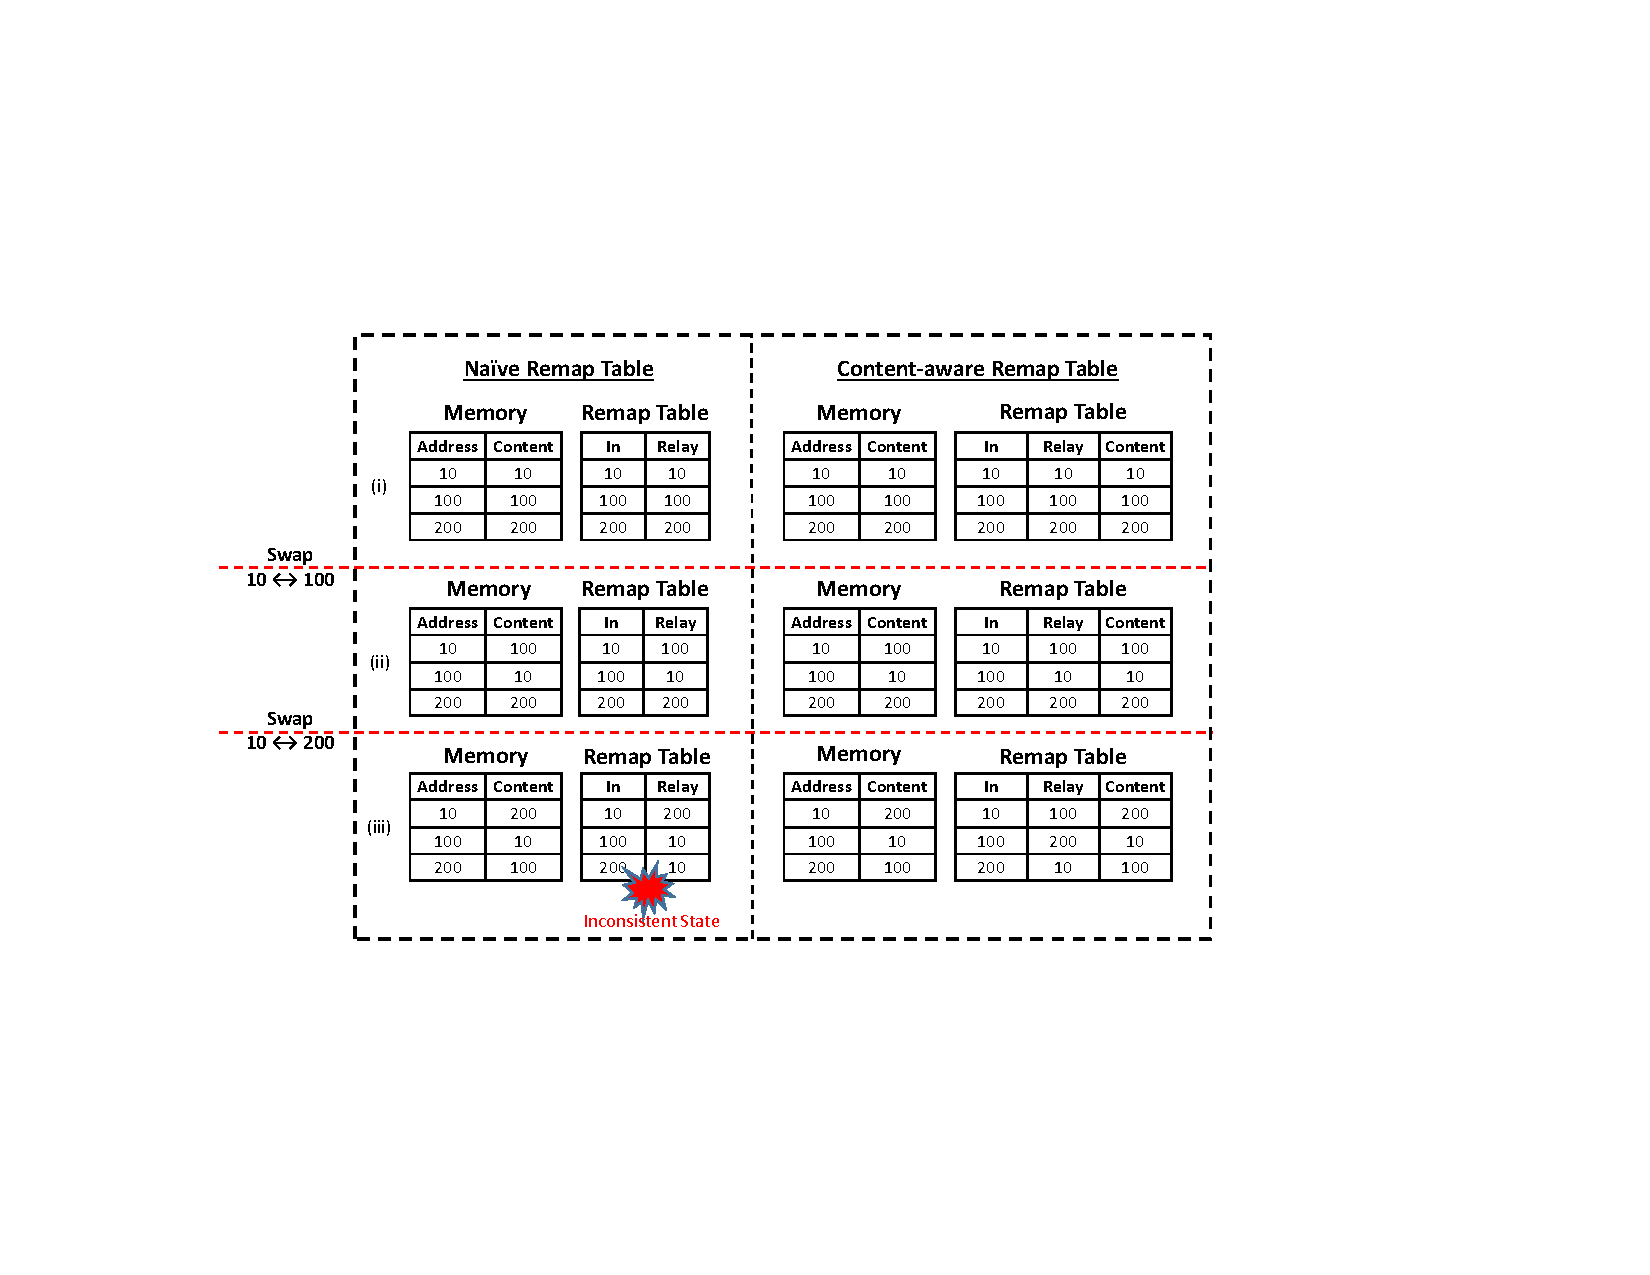
\includegraphics[width=0.46\textwidth]{figures/remap_table_design.pdf}
  \caption{Naive Vs content-aware remap table operation}
  \label{fig:remap_table_comparison}
\end{figure}

The first row shows the starting state of our memory before any migration, as well as the starting state of the two remap tables. For simplicity, we only present the three memory locations needed by our example. Page 10 is assumed to be a fast memory page, while pages 100 and 200 are slow memory pages. The numbers inside the memory locations represent the content page's id. The second row shows the states of memory and remap table after swapping pages 10 and 100. The content of page 10 is now page 100, and the content of page 100 is now 10. The naive remap table correctly states that requests to page 10 should be relayed to page 100 and vice versa. Everything works as it should during this first migration, however the third row shows the state after the second migration. Page 10 is now swapped with page 200. Such a migration would imply that page 100 (now held at 10) became cold and page 200 became hot. The contents are swapped and now page 10 holds page 200 and page 200 holds page 100. However, the state of the remap table is inconsistent. A request to page 10 would get forwarded to page 200, returning the wrong page. The right-hand side of Figure \ref{fig:remap_table_comparison} demonstrates the operation of a content-aware remap table able to support re-migration by updating the content page's remap table entry at each migration.

The naive remap table design fails simply because pages are allowed to re-migrate -- like page 10 in our previous example -- while the remap table ``assumes'' the content held at a page address matches the page's ID.  There is only one solution to this problem: The migration logic needs to be aware of exactly where each page's contents are located at any given time. Such a requirement can be implemented in various ways:

	\textbf{Safe and slow:} Always restore a forwarded page's contents to its original location before it participates in a new migration, resulting in two migrations instead of one. %For such an implementation, hot page count will have to be kept based on the content page instead of the real page Id. In the earlier example in Figure \ref{fig:remap_table_comparison}, the second migration of page 10 implies that page 100 is cold, but in order to offer page restoration support, the second swapping of page 10 will have to imply that page 10 is cold. The cold page (10) will be restored back to address 10 from 100 and then moved to its new location. Minor modifications are required to track activity based on the content page's id, that does not affect any other aspect of a migration mechanism.
}

	\textbf{THM approach:} Migration is restricted in ``segments''. In a memory configuration with a 1:8 fast:slow memory capacity ratio, each segment will have 9 pages; one in fast memory and the rest in slow. Each segment's 9 pages compete for a position at the one fast memory page available. This solution is elegant enough to allow re-migration with low storage overhead, limiting however the migration potential. If two or more hot pages coexist in a segment, only one can reside in fast memory at any given time. At the same time, if none of the segment's pages are hot, the fast memory page slot cannot be utilized by some other segment's page. %THM requires $\sim$5.6MB for its \textit{Segment Remap Table}.

	\textbf{HMA approach:} Any page can migrate to any other page address without the need of a dedicated remap table structure. The OS-based migration scheme imposes no limitations, as the OS takes care of updating the page tables and flushing the TLB. However, OS intervention and the penalties incurred due to cold TLBs can lead to high overheads.
	
	\textbf{MemPod approach:} Migration is restricted to be within a Pod,
Each Pod uses a remap table to allow page re-migration.  In addition to the
remap table, our algorithm also needs to identify all pages currently 
mapped to fast memory (to identify a candidate to be evicted in favor of a
new hot page).  We do this with a smaller, inverted table that gives the 
original address of each page currently mapped to fast memory.
 
%During the second migration in our example in Figure \ref{fig:remap_table_comparison}, the issue was caused because we updated the remap entry of the holding page (10) instead of the entry of the content page (100). An attempt to recursively follow the remap table's entries until we determine which one to update risks looping infinitely because of cycles (e.g., if page 10 is re-migrated back to address 10). Even if a smart algorithm is utilized to delete entries of non-migrated pages, the complexity of the recursive algorithm will only be bounded by the size of the remap table as, in the worst case, the entire table will be traversed. It's important to note that a content-aware remap table entry now points to a pair of values: (1) \textit{relay address} (where the requested page is located) and (2) \textit{content address} (which page is currently held). %MemPod requires 8MB per Pod and 32MB total for its sontent-aware remap table structure.

	\textbf{Alternative approach:} Recent works \TODO{Cite} propose the use of arbitrarily small remap tables. When the remap table inevitably fills up two possible solutions exist: (a) migration is disabled or (b) the OS is invoked to update page tables and flush the TLB. After OS's intervention, the remap table is cleared and migration remains active.
%\end{description}


%\begin{figure}[h]
%  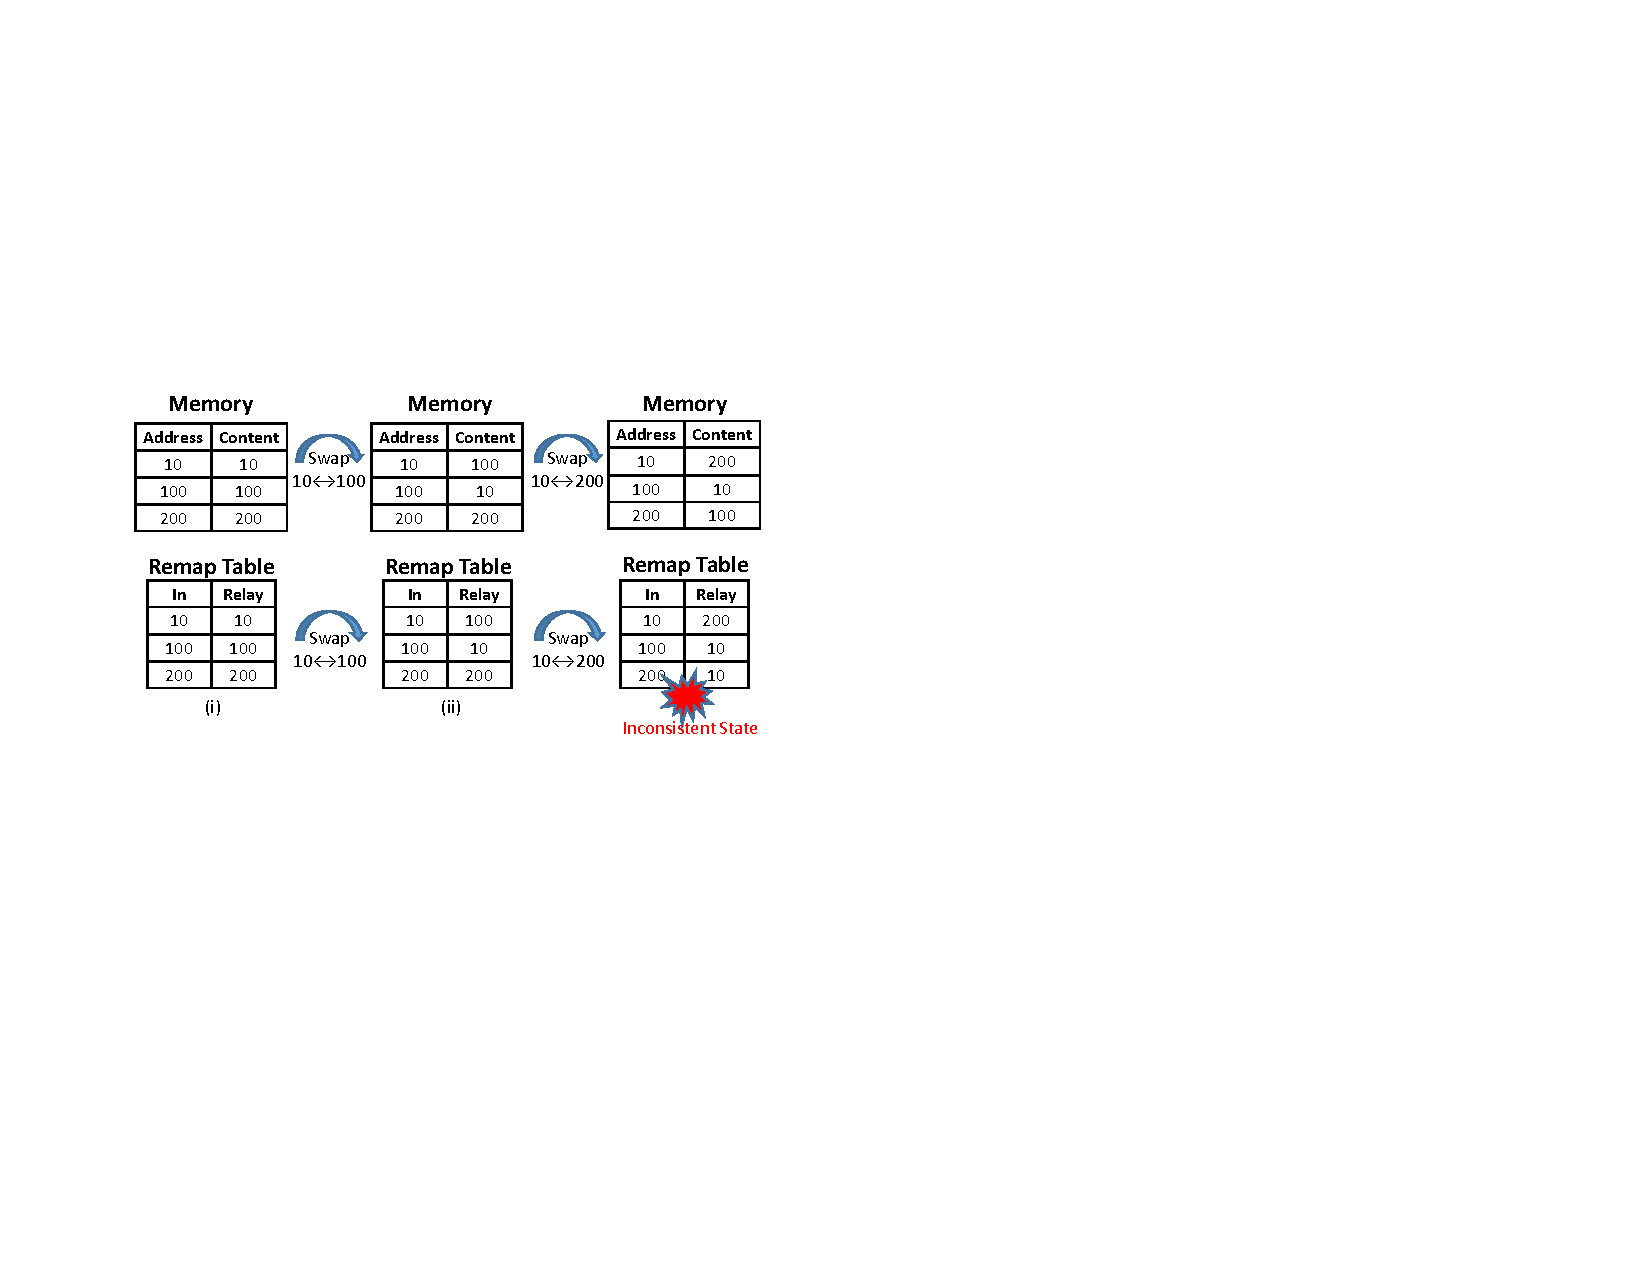
\includegraphics[width=0.46\textwidth]{figures/naive_remap_table.pdf}
%  \caption{Naive remap table operation}
%  \label{fig:failed_remap}
%\end{figure}
%
%\begin{figure}[h]
%  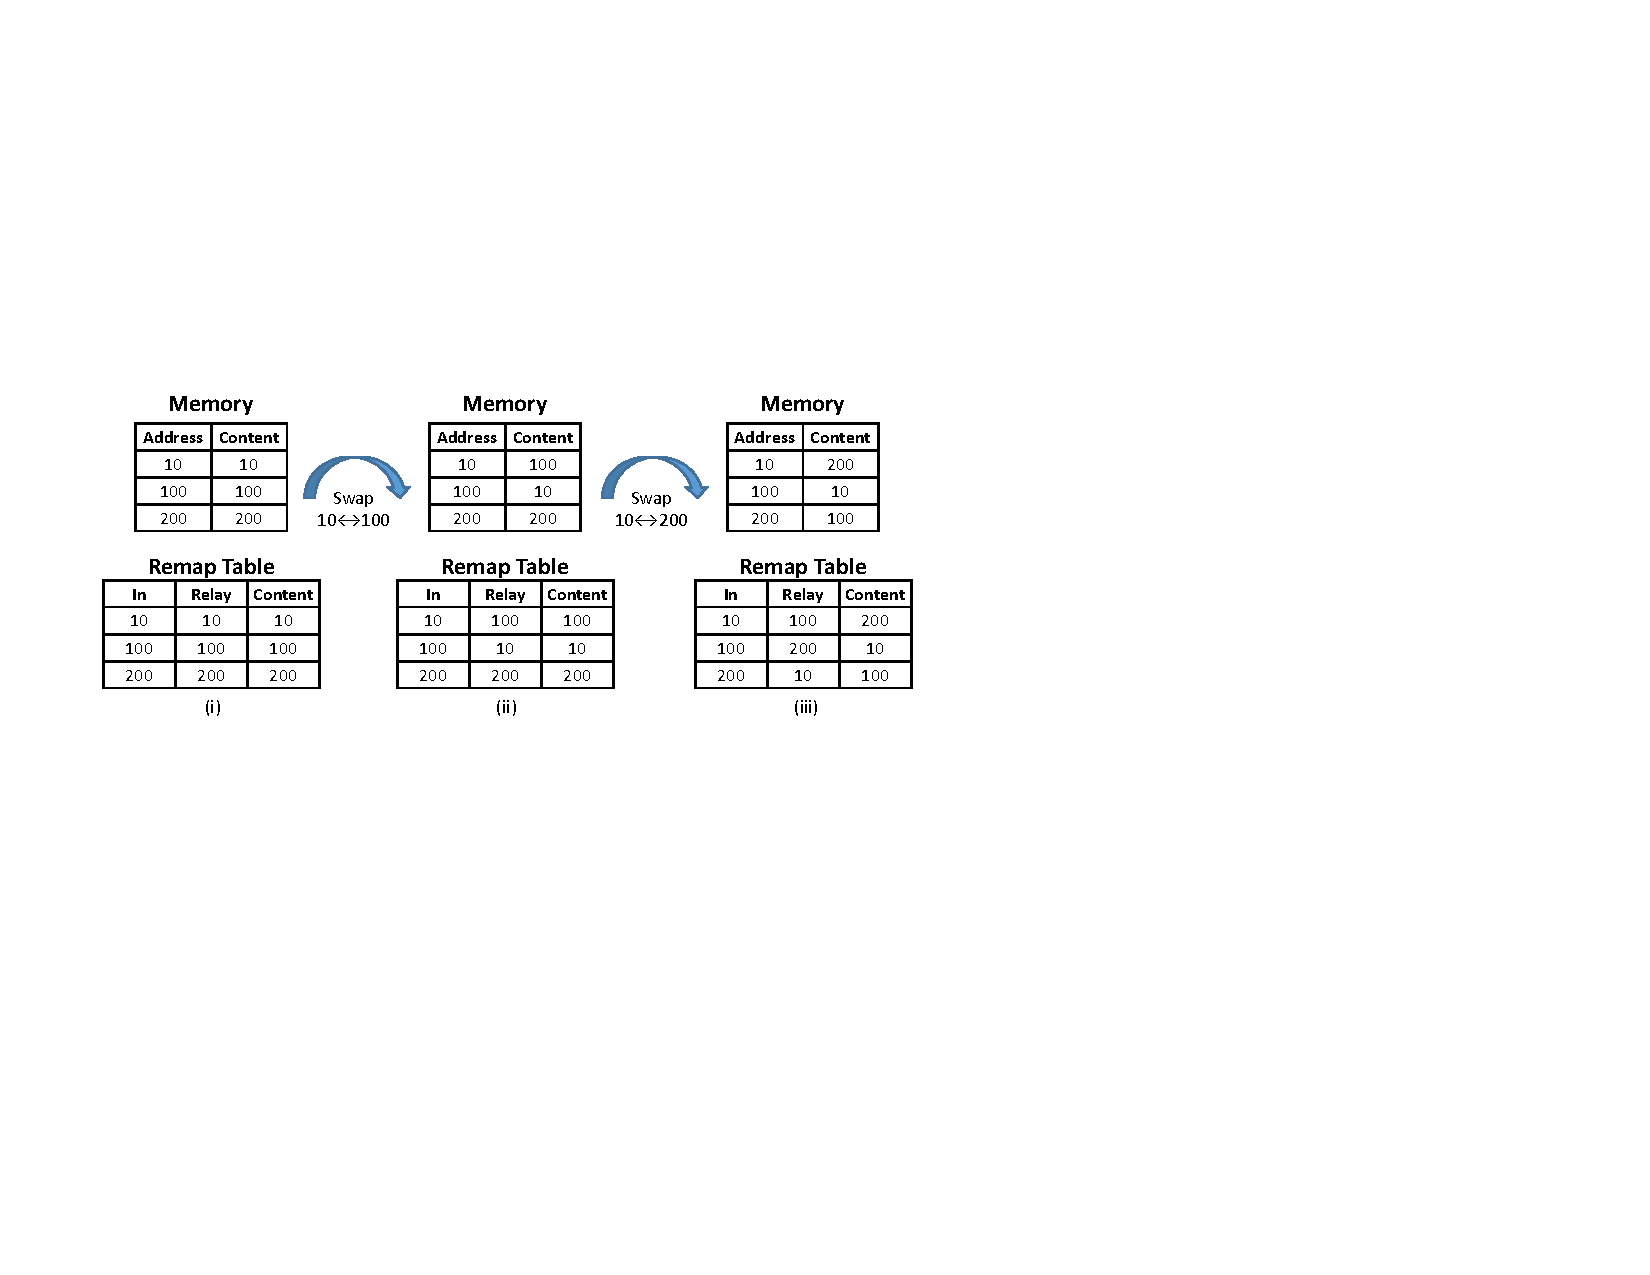
\includegraphics[width=0.46\textwidth]{figures/consistent_remap_table.pdf}
%  \caption{Remap design that allows re-migration}
%  \label{fig:correct_remap}
%\end{figure}


\subsubsection{Activity Tracking}
\label{sec:tracking}

Activity tracking could be considered the most important element of any management mechanism for hybrid memories. In most studies on the subject, activity tracking becomes a synonym for identifying hot regions by counting the number of accesses to each one. In a more generalized approach, it could potentially be extended to track patterns, parallelism, bit flips or any other information useful to the underlying mechanism. %Along with the remap structure, activity tracking is the limiting factor for most memory management mechanisms. The overhead of maintaining a set of counters per memory page (or any other granularity), is often a bottleneck. 

%MemPod utilizes an important observation to maintain a low activity tracking cost. Moving the hottest pages of an on-going interval into fast memory is a commonly accepted prediction technique, but not necessarily optimal. Several scenarios expose the failure of such an approach. For example, a page might become cold soon after it's migrated, wasting a space in fast memory. Another example arises when interval based migration policies are used. A cold page of the previous tracking cycle could become hot during the next interval. Strong indications exist that a combination of temporal as well as spatial locality has the potential of exposing better results. Our results in Section \ref{sec:MEA} demonstrate how Full Counters often conclude on a non-accurate prediction.

The overhead of maintaining a set of counters per memory page (or any other granularity), is often a bottleneck. Space requirements will increase linearly as memory capacities grow and the cost of sorting all the counters can overshadow any potential benefits in performance. Furthermore, our evaluation presented in Section \ref{sec:MEA} demonstrates that using full counters to ensure 100\% accurate counting may still lead to poor prediction accuracy. Frequently encountered cost-reducing solutions in the literature consist of increasing the activity tracking granularity in order to reduce the number of counters needed (i.e. track a group of pages together), limiting the bit width of counters, and caching a subset of the tracking state while the full set resides in main memory. 


%MemPod's activity tracking  is designed with a novel approach, using MEA to predict the hottest pages at a low cost. To the best of our knowledge, such an algorithm was never used in this context. THM also presents an interesting tracking approach, by utilizing competing counters for each segment.

%Using counters for every memory segment supported by the migration mechanism obviously imposes extremely high area overhead but benefits in \textit{counting} accuracy. Identifying the hottest pages however, also requires the often-overlooked sorting complexity. With the introduction of new memory technologies and the continuous capacity increase in memory capacities, it won't be long before even the most efficient sorting algorithm will require more time than we are willing to spend.

%\begin{description}
	\textbf{THM approach:} One 8-bit competing counter tracks each memory segment. A segment's competing counter is incremented by one when a page in its slow memory is accessed and decremented by one when the segment's fast page is accessed. The counter's value can then trigger migration when it exceeds a dynamically-set threshold. A ``monitoring region'' of memory where migrations are disabled is used by THM in order to update threshold values. Competing counters represent a trade-off between area overhead and accuracy and are susceptible to some error, as a cold page accessed at the right moment could trigger a migration and be placed in the fast memory.

	\textbf{HMA approach:} Full activity tracking per OS page (4KB) for all memory regions. HMA uses the least efficient tracking mechanism in exchange for perfect counting knowledge at a fine granularity. Full activity tracking also introduces the complexity of sorting all the counters to identify hot pages. THM and MemPod do not require explicit sorting.
	
	\textbf{MemPod approach:} MemPod requires an MEA map structure of K entries, where K is the number of hot pages we wish to identify at each interval. Our evaluation presented in Section \ref{sec:Results} determined the optimal number of MEA counters to be 128. Each entry maps a page's address to a counter. Through our evaluation, we identified the optimal counter size to be 4 bits and 62 bits are needed to address each page within a Pod, leading to a total of 1.03KB of space requirements. Using the MEA counters, MemPod's activity tracking profiles \textit{all pages in memory} at significantly reduced hardware cost. 
	
%As described in Section \ref{sec:MEA}, MEA is guaranteed to return the set of K hottest pages under certain assumptions that are not commonly held in a stream of memory requests. As demonstrated, MEA strikes a balance between most frequently occurring and most recently used page addresses, a fortunate and welcomed consequence in locality exposure. A new limitation arises when MEA counters are used: The system will be presented with the set of K hottest pages, however the counters' values cannot provide an order. The hottest page could have a lower counter value than any other page.
%\end{description}

Even with the most efficient tracking mechanism, future designs will soon be required to cache some of their counters while the rest are stored in main memory to alleviate the area overhead. THM's segment-based counters are automatically cached along with their corresponding remap table entries in THM's ``Segment Remap Table'' (SRT) and restored whenever necessary, at the cost of a memory access. As evident from the description in Section \ref{sec:MEA}, MEA cannot work well with a cache as it frequently needs to loop through \textit{all} entries of the map structure. However, the space needed by MEA is small enough to fit on chip and its size does not scale with increasing memory capacity, making it feasible to be used with future systems.

It is also important to note that activity tracking updates should be moved off the critical path. Extreme tracking accuracy is not necessary for correct operation of any migration mechanism. Even if the tracking mechanism is not as accurate as it could be, all memory requests will be able to retrieve correct information as long as the state of memory and remap structure are consistent. Updating a remap table entry however, needs to be performed accurately without any ambiguity to alleviate the risk of inconsistent state.

\subsubsection{Migration Triggers}

Deciding when to perform migrations is not always a trivial task. Migrations add significant delays to a system and, as such, they must be initiated wisely. Any penalties incurred should be amortized by the performance improvement from placing a page in the fast memory. Requests that arrive while migrations are being performed have to be delayed to ensure functionally correct memory behavior. Throughout the literature, two triggers are most commonly used whenever state must be updated based on tracking information (MC scheduling, migrations, dynamic voltage and frequency scaling etc.). Interval-based (or epoch-based) triggers occur with a set frequency, while threshold-based solutions trigger whenever a predetermined criterion is met. 

Both interval-based and threshold-based approaches face the same challenge of identifying the optimal interval or threshold value. Factors like a system's architecture, application's behavior, as well as semi-random factors (for example higher temperatures can lead to more frequent DRAM refreshes) make the optimal value differ from system to system. Designers usually opt for the value that provides the best results on average. The optimal value should not be too small as it will trigger some potentially expensive procedure frequently, but it cannot be too large as that reduces the ability to adapt to application phase variations. 

%As far as memory migration in flat address spaces is concerned, the state-of-the-art mechanisms trigger their migration procedures based on:
%\begin{description}

	\textbf{THM approach:} THM uses a threshold-based mechanism. When the competing counter described in section \ref{sec:tracking} exceeds a threshold value, migration is triggered. THM will swap the page that triggered the event with the page currently residing in the segment's fast memory page. Each segment can trigger migration independently and asynchronously since no interval is used. THM risks very frequent migrations that will stall the stream of incoming requests until each swap is finished. To overcome this issue, THM dynamically predicts the expected benefit of using one threshold value from a set of four pre-defined values. A ``sampling region'' of memory where migrations are disabled is used allowing THM to extrapolate and associate a potential benefit with each one of the pre-defined threshold values. When THM expects that migration costs will be amortized it updates the threshold value.
	
	\textbf{HMA approach:} HMA uses an interval based mechanism. Upon each interval, HMA attempts to migrate enough pages to fill the entire fast memory. However the high cost associated with OS intervention, management and the penalties of cold TLB favor long intervals. HMA authors identified the optimal timing interval to be as high as 1ms.
	
	\textbf{MemPod approach:} MemPod uses timing intervals. At each interval each Pod will migrate up to K pages into the fast memory, where K is the number of MEA counters used. MemPod is transparent to the system, rendering costly OS intervention unnecessary. Since each one of the N Pods will attempt to migrate up to K pages, up to N$\times$K migrations can happen within each interval. However, all Pods can perform their migrations in parallel. %The time required by MemPod to execute N$\times$K migrations is equal to the time to execute K migrations.
	
%\end{description}

\subsubsection{Migration Driver and Decentralization}

Multiple channels, each with its own MC, in modern memory organizations expose channel-level parallelism. Each channel can service requests independently. Some migration mechanisms in the literature inherently ``assume'' a centralized migration controller in charge of monitoring traffic, while others attempt to implement a completely distributed mechanism. A centralized approach can be severely limiting. Current HBM memory technology allows up to 8 channels per stack \cite{JEDEC-HBM-REVISED}, while many processors are already designed with four or more off-chip memory channels. Our evaluated system in this paper features a total of twelve memory channels. Channel number is predicted to increase in the near future \TODO{[cite]}. Channel parallelism capabilities will be greatly hindered if we enforce request serialization due to migration-related activity tracking or remap table lookups. On the other hand, a fully distributed solution will eliminate all serialization, at the cost of any-to-any communication among channels. An alternative to the communication cost would require OS intervention. MemPod's novel clustered architecture attempts to balance this tradeoff. 

As with most of the essential elements for migration presented in this Section, the system's designer can choose any level of centralization desired according to the specific design's constraints. As such, the body of migration research covers the entire range:
%\begin{description}

	\textbf{THM approach:} Even though not clearly stated in the THM paper, it appears the authors opted for a centralized unit and consequently all channel parallelism potential is lost, placing THM last in our list in terms of parallelism potential. Decentralizing THM's migration controller appears to be possible, but in that case cache coherency becomes a concern as THM caches its remap table and competing counters structure. Race conditions could occur if the same SRT entry is simultaneously cached in different locations and its counter is modified. To ensure a fair comparison in our evaluation of THM, we assumed it can utilize the full channel-level parallelism potential of a system. 
	
	\textbf{HMA approach:} HMA ranks at the top of our list in terms of parallelism, featuring a fully decentralized mechanism. It's important to note that HMA does not require a remap table and consequently one possible source of request serialization is automatically removed. Activity tracking is performed at each MC individually (requiring hardware support), where each controller will monitor the activity of its own pages. When HMA's migration is triggered, the OS will collect all activity monitors from all the MCs before it proceeds with migration. Collection of this information from each MC by the OS is likely to consume a considerable number of cycles.
	
	\textbf{MemPod approach:} Clustering memory channels into Pods comes with significant benefits. First, assigning exactly one off-chip (slow) memory channel to each independent Pod ensures those channels can still service requests in parallel. Being the slowest part of our memory hierarchy, keeping slow channels independent does not add delay to a potential bottleneck. Furthermore, each group of two on-chip (fast) channels can still operate in parallel. Some serialization is introduced between sibling fast channels. However with a Pod's light-weight design and the high bandwidth of HBM channels, the delay is minimized. Beyond channel parallelism, each Pod can hold all the migration-related structures, eliminating the need to retrieve information from each MC at each migration interval.
	
%\end{description}

\subsubsection{Migration Datapath}

Regardless of the choice for each migration building block described so far, once migration is triggered, any migration manager has to follow the same steps. First, migration candidates need to be identified. Traditionally, one page (or a segment depending on the migration granularity) from the slow memory and one from fast memory. The two identified candidates need to be swapped. First one or both pages will be read and stored in temporary buffers and then written at their remapped locations.

Describing the actual migration datapath is often overlooked in migration publications. Without dedicated page migration driver hardware, migration will have to be orchestrated by the OS and CPU cores. Consequences include communication delay, potentially some delay introduced at the processor's cache levels and the performance degradation caused by the unavailability of those CPUs during migration. 

MemPod implements the migration driver within each Pod. As the Pod has direct communication with the MCs, added delays are kept to a minimum, no traffic is generated at the global switch saving energy and the CPUs are free to keep executing non-memory instructions. In HMA, the OS orchestrates everything. Some CPU cores have to be stalled and used to service the OS interrupt, causing the migrated pages to traverse through communication mediums and caches on each way. THM does not describe its datapath in detail and it appears that CPUs are used in this case as well. For fair comparison, we do not model the penalty introduced by using CPUs for migration in our HMA and THM simulations presented in Section \ref{sec:Results}.

%We assume that channel parallelism is utilized when reading and writing the candidate pages. In other words, the two read commands will be sent in parallel, as well as the write commands that follow. Consequently, The hardware penalty for one page swap is the time required to read an entire page from and then write it to the slow memory. We also assume that writing the two candidates back incurs row buffer hits since the page was just opened in the previous step. In this study, we evaluate all mechanisms under the same memory organization and as such, the memory time required for one migration is the same across all mechanisms. However, each mechanism introduces some unique penalties:
%\begin{description}

	\textbf{THM} does not introduce a cost for identifying the candidate pages as it follows a deterministic algorithm. The page that caused the competing counter to exceed the set threshold will be the slow memory candidate, while there is exactly one fast page candidate per segment.

    \textbf{HMA} attempts to fill the entire fast memory with migrated pages. The number of swaps that will be performed per interval can be as high as the number of pages in fast memory. Inevitably some hot pages will already reside in the fast memory and they will not be migrated to a different location in fast memory. HMA introduces costs that are hard to estimate. Sorting all the activity tracking counters, traversing and updating page tables and flushing TLBs are all parts of the cost introduced by the OS. In addition, the effect of cold TLBs can severely penalize all running applications. %We modeled HMA to not attempt migration of those hot pages. Such an approach could complicate finding a fast-memory candidate page, although with HMA's full activity tracking counters, and since sorting is a necessary operation at every interval, this problem can be reduced to the simple task of following the sorted activity list backwards (i.e. It's easy to find the coldest fast-memory page). Unfortunately, HMA introduces costs that are hard to estimate. Sorting all the activity tracking counters, traversing and updating page tables and flushing TLBs is part of the cost introduced by the OS. On top of that, the effect of a cold TLB can penalize severely all running applications.

	\textbf{In MemPod,} with the use of MEA counters, identifying the fast-memory page candidate is as simple as checking that it's not part of the K hot pages. The identification algorithm starts at the very first fast memory location and iterates sequentially until it detects a page address that is not in the set of hottest pages. For the next migration, the identification algorithm simply continues from where it was left. If a hot page already resides in the fast memory it's ignored.
%\end{description}

\subsection{Scalability to Future Memories}

\remark{Nuwan's comment:\\I feel like this section has a lot of repetition from what was already stated earlier in this section. It could either be shortened quiet a bit or removed (but if we remove it, we need to make sure the references earlier in the paper about how we expect MemPod to be better for future memory systems aren't left dangling).}

As main memory capacities grow to terabytes, storing activity tracking information and remap tables in SRAM could become infeasible. Caching part of the migration logic and using part of main memory as backing storage will become necessary. MemPod's semi-distributed architecture allows caching without any coherence concerns as Pods never share information. %An analysis on the impact of such caching, as well as the optimal cache size is presented in the experimental evaluation section. 

At such capacity levels, centralized migration controllers will no longer be sustainable due to the severity of the introduced request serialization penalty. Further, as applications become more data-centric, it's safe to assume that memory traffic would also scale up, as well as sustainable bandwidth expectations. 

Alternative approaches described in this Section limit the size of the remap table at the cost of disabling migration when full, or invoking the OS before migration resumes. This approach could also be incorporated in future migration mechanisms. We should note that with a limited remap table size, or even an available number of counters less than the number of fast pages, MemPod would still offer the potential of migrating \textit{any} slow memory page to the limited set of fast pages (as long as it's within the same Pod) available for migration, in contrast to THM, where only those segments that happened to fit in the new limited size will be able to migrate, forbidding migration of the rest of the slow pages. HMA would remain intact from this limitation since no remap tables are necessary.



















































